\begin{figure}
    \centering
    \begin{subfigure}{\linewidth}
    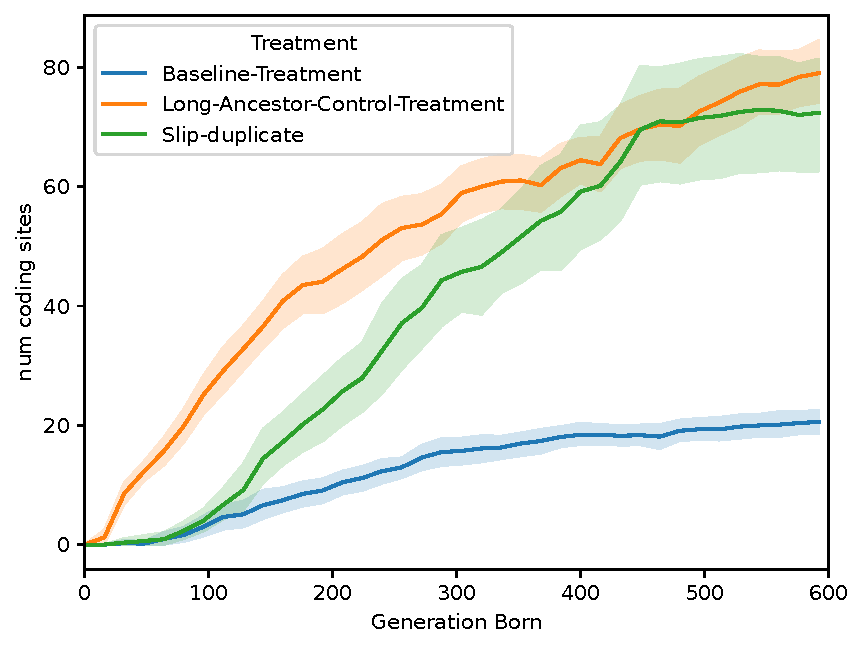
\includegraphics[width=\linewidth]{binder/binder/teeplots/hue=treatment+post=plt-xlim-0-600+viz=lineplot+x=generation-born+y=num-coding-sites+ext=.pdf}
    \caption{\footnotesize active coding sites}
    \label{fig:num-coding-sites:coding}
    \end{subfigure}

    \begin{subfigure}{\linewidth}
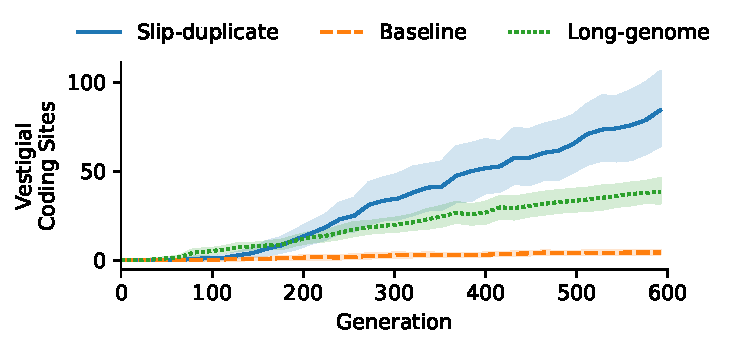
\includegraphics[width=\linewidth,clip, trim=0 0 0 0.8cm]{binder/binder/teeplots/hue=treatment+post=plt-xlim-0-600+viz=lineplot+x=generation-born+y=num-free-sites+ext=.pdf}
    \caption{\footnotesize vestigial coding sites}
    \label{fig:num-coding-sites:coded}
    \end{subfigure}
    \caption{
        \textbf{Accumulation of active and vestigial coding sites.}
        \footnotesize
        Generation-by-generation counts of coding sites over evolutionary history.
        Here, ``active'' coding sites refer to genome instructions determined through knockout to contribute to fitness with respect to self-copy viability or a logic-9 phenotypic trait.
        Vestigial coding site count, by contrast, reports the number of sites determined to have contributed to fitness in an ancestor, but are no longer active coding sites.
        Error bands give 95\% CI, bootstrapped over 30 replicates per treatment.
    }
    \label{fig:num-coding-sites}
\end{figure}
